\documentclass{article}
\usepackage{titling}
\usepackage{lipsum}
\usepackage{amsmath}
\usepackage{listings}
\usepackage{graphicx}
\usepackage{subcaption}
\usepackage{pgfplots}
\usepackage[margin=1in]{geometry}
\usepgfplotslibrary{statistics}



\begin{document}
\noindent
\begin{minipage}[t]{0.6\textwidth}
    \begin{flushleft}
        \LARGE\textbf{Math 343 - Lab 5} \\
        \vspace{6pt} % add 6pt of vertical space
        \hrule width 10cm
        \vspace{12pt}
        \large\textbf{Preston Duffield} \\
        \large Western Washington University \\
        \today
        % April 18, 2023
        \vspace{24pt}
    \end{flushleft}
\end{minipage}

\section*{Question 1}
\subsection*{a)}
To estimate value of $(\tau \beta)_{22}$, first must observe that
$\bar{y}_{2 2 \cdot} = \frac{100 + 85.9}{2} = 92.95$.
$\bar{y}_{2 \cdot \cdot} = 85.9$.
$\bar{y}_{\cdot 2 \cdot} = 100$.
$\bar{y}_{\cdot \cdot \cdot} = \frac{100 + 79.2 + 85.9 + 83.9}{4} = 87.25$. \\

Therfore: $(\hat{\tau \beta})_{22} = 92.95 - 85.9 - 100 + 87.25 = -5.7$
\subsection*{b)}
First we note the following: \\
$\hat{\mu}_{11} = 83.9$ \\
$\hat{\mu}_{12} = 85.9$ \\
$\hat{\mu}_{22} = 100$ \\
$\hat{\mu}_{21} = 79.2$ \\
The main effect of source of protien (A) is: \\
$\frac{79.2 + 100}{2} - \frac{83.9 + 85.9}{2} = 4.7$ \\

The main effect of amount of protien (B) is: \\
$\frac{85.9 + 100}{2} - \frac{83.9 + 100}{2} = 1$ \\

The interaction effect of the two sources is: \\
$\frac{100 + 83.9}{2} - \frac{79.2 + 85.9}{2} = 9.4$ \\
\subsection*{c)}
\begin{figure}[h]
    \centering
    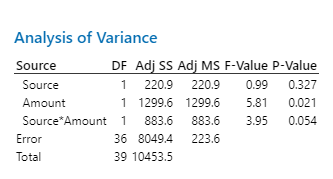
\includegraphics[width=0.5\textwidth]{./images/1_c.png}
    \caption{The ANOVA table from Minitab.}
    \label{fig:1_c}
  \end{figure}

\subsection*{d)}
\subsubsection*{i.}
\subsubsection*{ii.}
\subsubsection*{iii.}
\subsubsection*{iv.}
\subsection*{e)}

\section*{Question 2}
\subsection*{a)}
\subsection*{b)}


\end{document}
